\section{Implementation Steps} \label{sec_implementation_steps}

At the end of the project, there were two alternative pipelines. These pipelines are depicted in Figures \ref{fig_pipeline_1} and \ref{fig_pipeline_2}.

\begin{figure}[h]
    \centering
    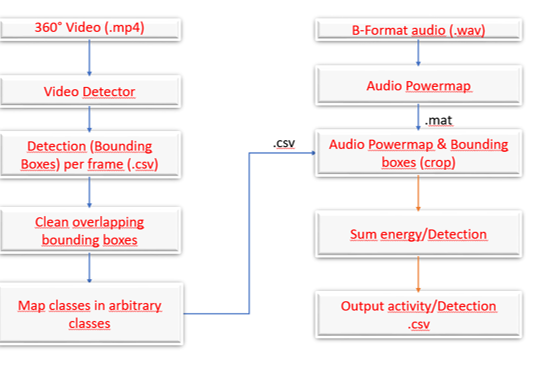
\includegraphics[width=0.95\textwidth]{figures/pipeline_1.png}
    \caption{First variant of the project pipeline.}
    \label{fig_pipeline_1}
\end{figure}

In the first variant of the pipeline (Figure \ref{fig_pipeline_1}), the 360-degree video is first used as an input to a video detector...

\highlight{(some more description about the video detector and the CSV output here, also mention something very shortly about YOLOv4 and use its reference \cite{yolov4_paper})}

Then, when the video detections have been acquired, it can be observed that there are multiple overlapping bounding boxes for detections of the same class instances. Therefore, a function which cleans overlapping bounding boxes was implemented. The basic idea of the iterative bounding box cleaning function is the following:

\begin{enumerate}
    \item If there are same classes present in a video frame, then proceed to part 2.
    \item If the detected bounding boxes of the same object classes are overlapping more than a predefined threshold, then proceed to part 3. The overlap is determined by the intersection over union.
    \item Remove the bounding box with the least confidence as determined by the visual object detector.
\end{enumerate}

After cleaning the CSV file of overlapping bounding boxes, it is possible to map any given class or classes from the object detector into a new arbitrary class. For example, all types of vehicle object detections can be mapped into a new class calld `vehicle'. For this, a class mapping function was created.

Up until now, all descriptions have focused on the video detection side. For the B-format audio (4 channels) obtained from the microphone array, a function provided by one of the clients (Archontis Politis) converts the audio into a powermap representation using the MUSIC (MUltiple SIgnal Classification) algorithm. Then,

\highlight{(description about cropping audio powermaps, converting into azumuth and elevation etc.)}

\begin{figure}[h]
    \centering
    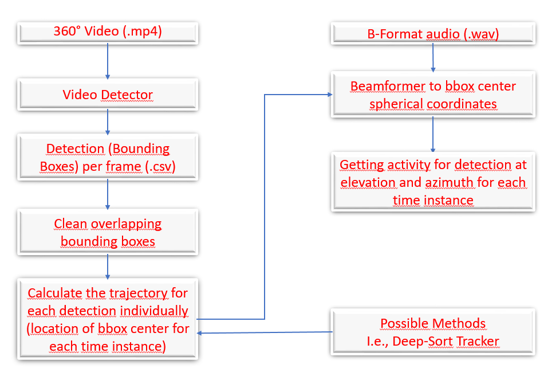
\includegraphics[width=0.95\textwidth]{figures/pipeline_2.png}
    \caption{Second variant of the project pipeline.}
    \label{fig_pipeline_2}
\end{figure}

In the second variant of the pipeline (Figure \ref{fig_pipeline_2}), the initial parts of the video processing side are the same as in the first variant of the pipeline. Now, the B-format audio is not converted into an audio powermap. Instead, the audio is used as an input to a \textit{beamformer}, whose code was also provided by one of the clients (Archontis Politis). The beamformer basically ``listens" to a given direction. In our case, this direction should be the direction of a given object.

What turned out to be problematic for the beamforming was that it is difficult to determine associations between objects in a given scene, e.g. is a given object instance one of the object instances of the same class in the previous video frame. Therefore, two alternate cases were implemented: 1) Audio segments of multiple video frames, and 2) Audio segments of a single video frame are used as an input to the beamformer.

When inputting audio segments corresponding to multiple video frames, the pre-processing code was simplified so that only one object could be present in a given video scene. The temporal trajectories of this given object were then determined so that if the object was appearing for more than four consecutive video frames, then its temporal trajectory was taken into account. If the object did not appear for more than four consecutive video frames, then its temporal trajectory was discarded. After obtaining the temporal trajectories of the given object in a scene, the sound segments and the frame-level bounding box centers (converted into azimuth and elevation in radians) that correspond to a given temporal trajectory were given for the beamformer to produce a spectrogram-like energy representation for each audio frame of the object. Finally, if the sum of the frequency bin-level energies exceeded a predetermined threshold, the audio frame was said to contain audio activity. Furthermore, since the audio frames had a different framerate than the video had, the audio activity detections were determined based on the sums of the bin-level energies that were interpolated into a 10-fps framerate.

In the other variant where the audio segments of single video frames being used as an input to the beamformer, all objects within a video frame were first listed. Then, for each object detection in a video frame, the location (azimuth and elevation of bounding box center) and the corresponding audio segment (100-ms segment for 10 fps video) were used as an input for the beamformer. For the spectrogram-like energy representation produced by the beamformer, the total energy of all frequency bins was summed. If this sum exceeded a predefined threshold, then the visual object was determined to have audio activity in the given video frame.

To get more intelligent temporal trajectories of visual objects, visual object tracking methods should be applied. An example of a visual object tracker is Deep SORT \cite{deepsort}. Deep SORT is one of the simplest algorithms used in object tracking. It is used for tracking multiple objects in real-time applications. Like the SORT algorithm, the Deep SORT algorithm uses the Kalman Filter method to predict the location of objects in the next image. Deep SORT and SORT algorithms are separated from each other by the method they use when associating objects. A convolutional neural network (CNN) is designed for object classification to be used in the Deep SORT algorithm. The convolutional neural network is trained until high accuracy is achieved. Thanks to CNN, the most distinctive feature of the object to be classified, and the most distinctive feature that distinguishes the object from other objects, is tried to be determined. In the last layer of the CNN structure, the classification of the objects is done. This classification process is done according to a vector representing the object. In the Deep SORT algorithm, a vector is obtained by passing each detected object through the neural network and using these vectors to associate the two objects. This vector is called the "appearance feature vector" According to the SORT algorithm, the Deep SORT algorithm is more successful in object association in cases such as occlusions since it is more specific and distinctive features of the object are examined to associate an object with another object.

To test the methods during development, small test scenes were constantly recorded during the project using the 360-video camera and the microphone array. At the end of the project, all three group members gathered at the university to produce carefully planned recordings to demonstrate and highlight functioning as well as non-functioning parts of the pipeline.



\section{Meetings, Week Reports and Inspections}

During the project, almost every Friday at 14:00 a MS Teams meeting was organized together with the clients to discuss updates about the project from the past week, and to set goals for the following week. Additionally, communication with the clients was carried out via MS Teams and email.

\section{Deliverables}

The main deliverables of the present project were the source codes and their thorough documentation created during the project which are provided in a GitHub repository. Additionally, the present final report is the main deliverable course-wise.

\section{Timetable and Workload}

As was originally planned, the project proceeded according to what was agreed on each weekly Teams meeting with the clients, with the aim to complete the given tasks during the following week. After each Teams meeting, the group members discussed about the division of the workload so that each member would have approximately the same workload as other group members.

There was no specific weekly timetable planned for the project before the start of the project. The main timetable was that at least one functioning version of the task pipeline should be finished by the end of the course, which was achieved successfully. Furthermore, we were even able to provide an alternate functioning version of the pipeline.

\section{Budget}

For achieving the project goals, approximately the time planned in the initial project plan was used to the project. That is, approximately 133.3 working hours for each group member. By assuming that all group members would be recently graduated M. Sc. (Tech.) workers with the recommended starting salary by TEK (the largest organization for academic engineers in Finland) which is 3980{\euro}/month, the project would cost approximately 9256{\euro} altogether.

The two clients used approximately 30 minutes for each remote meeting which occurred almost every Friday (for calculations, we can assume that the remote meeting occurred every Friday). In addition, if it is estimated that the clients both use approximately 30 minutes for the project each week outside the meeting time (such as reading and answering to messages on MS Teams), this gives an additional two working hours each week for the clients. Furthermore, one of the clients used time to provide code for the project group. If we assume that this contribution would take one hour on average for each week, we would have that altogether the clients used approximately , this leads to approximately 42 working hours for the clients. This is significantly over the initially estimated 28 hours (50\% more). If an estimate of the salaries of the clients would be e.g. 5000{\euro} a month, then their input to the project would cost approximately 1221{\euro}.

\section{Problems, Delays and Changes in Project Organization and Plans}

During the project, there were no major issues hindering the progress of the project. However, out of the original project plan, testing the implementation against manual annotation was not put into practice. This was due to the fact that instead of only finishing one possible version for the project pipeline (audio powermaps), another version of the pipeline (beamforming) was also implemented. This additional version was not planned during the beginning of the project, and it was proposed near the end of the project by the clients.

\section{Lessons learned}

What was noticed during the project was that without a visual object tracking method, it is extremely difficult to define correspondences of objects across video frames. In addition, although there are multiple different types of projections (e.g. stereographic or perspective projection) to convert a curved equirectangular image into a less curved version, it was observed that practically all of these projections have their pros and cons, and no projection is able to perfectly convert an equirectangular image into an ``ordinary" image. For example with the stereographic projection that was used in the present experiments, it was observed that objects that are very close to the camera (and therefore very curved) are not well detected by the video object detector, even though a stereographic projection is applied to the equirectangular image before using the video detector. Furthermore, what stood out as new information was that it is not possible to get an accurate sound localization using only four microphones, although four microphones might sound like a lot for conventional applications.

\highlight{(More lessons learned here)}

\section{Future Development Needs} \label{sec_future_development_needs}

There are several ways to improve the presented implementations. First, the implementation should be tested more vigorously. For example, now there were only five well-designed indoor scenes recorded, whereas a greater number of recordings, both indoors and outdoors, should be recorded to better highlight the pros and cons of the present pipeline. Also, the outputs presented implementations should be tested in actual sound event detector training to showcase that how do the automatically generated labels perform in real-life use cases.

For improving the video detector side, the present pre-trained video detector is only able to detect a little over 80 visual objects, out of which the majority (e.g. pizza, frisbee, parking meter etc.) are not useful at all for representing sound-making objects. The video detector could further be developed by only training it with objects that are useful for the present task. In addition, it was observed in the test scenes that if some object is very close to the camera, it is not detected from the equirectangular image, although the video processing pipeline handles curved visual objects on some level. Therefore, either the video detector should also be trained with images that are warped a little, or the recorded scenes should be designed more carefully so that objects are not very close to the camera. Furthermore, even though a 4k resolution that the Ricoh Theta V camera produces is a rather good video resolution for conventional video, in fact a 4k resolution is considered to be a small resolution in 360-degree video. To better detect objects (especially objects that are far away from the camera), a camera with a better resolution should be used.

To better improve the audio processing side, both the audio powermap and the beamforming could be improved by trying out the system with a microphone array with a better spatial resolution, i.e. more microphones should be used (only four microphones were used in the present experiments). Also, the present audio processing implementations require that sound-making objects should not be very close to each other. This could also be improved by using microphone arrays with more that four microphones. To further improve the beamforming method, video tracking methods should be used together with the object detector to intelligently produce time arcs of visual objects in a scene.

Finally, the present proposed pipelines work piece-by-piece, but are not designed to function in an end-to-end manner. To make producing audio event labels easier, the proposed pipelines could be made end-to-end so that the final output CSV could be produced e.g. by inputting an MP4 video file with B-format audio into a program together with some configuration file which determines the details about the way the user wants to produce the audio event labels.


